\chapter{Transfer Learning}
\label{ch:transfer_learning}

\begin{remark}{Outline}
	We now present Transfer Learning (TL), a machine learning methodology that aims to create algorithms capable of retaining and reusing previously learned knowledge when getting trained on new, unseen problems. Most of the contributions presented within this dissertation are motivated by TL. Therefore, we now introduce the readers to this specific learning paradigm to provide them with all the preliminary knowledge necessary to fully understand the research presented in the coming chapters. We start with a gentle introduction to TL in Sec. \ref{sec:tl_introduction} where we describe the main concepts underlying TL and explain why it is desirable to have machine learning models that are transferable. We then show in Sec. \ref{sec:rationale} some practical, high-level examples that visually represent the benefits that can come from adopting TL strategies in machine learning. We will then provide more rigorous mathematical definitions in Sec. \ref{sec:definitions} where we will characterize TL both for the supervised learning setting as well as for the reinforcement learning one. In Sec. \ref{sec:literature_review} we thoroughly review how TL has been studied by the deep learning community in both settings. We end this chapter with Sec. \ref{sec:relevance}, where we describe how all the machine learning concepts encountered throughout the first part of this dissertation will play a role in the coming chapters.  
\end{remark}

\section{Introduction}
\label{sec:tl_introduction}
Imagine being an Italian Ph.D. student living abroad who just went for dinner with his French housemate. You had the chance of eating the best, most Italian pasta the two of you have ever eaten in almost ten years spent abroad. The pasta was so good that, one week later, you cannot see yourself as having anything else for dinner. Unfortunately, when your housemate suggests going back to the restaurant, you have to politely decline the invitation, as your favorite Italian restaurant, next to serving delicious food, is also extraordinarily expensive. This prevents you from going there at least until the end of the month, which is when your gentle supervisor will kindly pay you despite you not having published a single paper in over a year. However over all the years you spent abroad, seeking some proper Italian food that was supposedly going to make you feel less homesick, you learned how to cook plenty of pasta yourself. The outcome of your cooking sessions is certainly not on par with those of your favorite restaurant, but over the years, resulted in some pretty tasty dishes nevertheless. Therefore you decide to cook dinner for yourself and your housemate by replicating the pasta you had as dinner one week ago. While cooking, you try to remember all of the knowledge you acquired over the years while learning how to cook abroad. You remember how to salt the water properly, how long to keep the pasta in the boiling water, and how to season the sauce with the right mix of spices. In the end, the resulting meal, albeit not perfect, will turn out to be a much better dish than the one you will be having one week later, when, this time, it will be your housemate's turn to replicate the pasta for dinner. The reason your pasta ended up being tastier than your housemate's is not that your housemate is French, but rather because he turned out to never having cooked any pasta before. Therefore, he had no previous knowledge to attain from while cooking, while you could instead re-use a set of previously acquired cooking skills. This intuitive but straightforward life episode perfectly summarizes the concept of \textcolor{RoyalBlue}{Transfer Learning}, the main topic of interest of this dissertation. However, throughout this work, we will not be focusing on any sort of cooking abilities, nor on any Ph.D. student other than the one authoring this document. We will instead center our attention on situations where it is particularly desirable to have machine learning models, particularly neural networks, that are transferable. 

\subsection{Transfer Learning in Machine Learning}
There are many reasons that can motivate why it should be worth studying machine learning models from a Transfer Learning (TL) perspective. In this dissertation we have mainly been driven by the following rationale. A first typical scenario where it is helpful to have transferable models is characterized by the \textcolor{RoyalBlue}{lack of training data}. This is a problem that mostly affects supervised learning and is typical of situations where collecting and annotating data is an expensive and laborious task (we will see one of such situations in Chapter \ref{ch:tl_lth}). As we have seen in Chapter \ref{ch:supervised_learning}, the ultimate goal of supervised learning is that of training a machine learning model that minimizes the empirical risk alongside the expected risk. Unfortunately, when training data is limited, it is well known that this goal becomes much harder to achieve, as the resulting learning algorithms become more prone to overfitting and successfully training neural networks can therefore become problematic \cite{aggarwal2018neural}. 
TL is also particularly desirable when there are \textcolor{RoyalBlue}{limited computational resources} available, which might not allow machine learning practitioners to train new models each time a novel machine learning task is encountered. This can be the case both when tackling supervised learning problems as well as reinforcement learning ones, although we believe that among the two learning paradigms, the resources that are required by reinforcement learning are by far more prone to becoming out of reach for many researchers (for a position paper about this topic, we refer the reader to the work of \citet{obando2020revisiting}).
Lastly, we also believe that studying the degree of transferability of machine learning models has potential additional benefits that go beyond the aforementioned practical advantages. In fact, we argue that TL offers an effective tool for \textcolor{RoyalBlue}{better understanding} the machine learning models that are currently being used. By analyzing whether such models can be adapted to novel unseen tasks, it is possible to gain insights about their generalization capabilities, as well as their fundamental inner workings.


\section{Transfer Learning in Practice}
\label{sec:rationale}

%Before mathematically defining TL, we continue building some intuition by visually representing how one can observe the benefits of TL in practice. We assume that we would like to solve a certain task and that we can choose between two different models: a model that has never dealt with any task before, and a second model, which is identical to the first one with the major difference being that it has already seen a similar task in the past. Because of their different nature, we refer to the first model as a model trained from scratch and to the second model as a pre-trained model. Ideally, as mentioned in the previous section, we would like the latter model to perform better on the considered task than the first one. Yet, how can we assess if one model is better than the other one? As initially presented by \citet{langley2006transfer}, and later generalized by \citet{lazaric2012transfer}, we would like the performance of a pre-trained model to result in three possible improvements. If at least one of these improvements is observed while training, we can then consider the pre-trained model to be a better alternative than the scratch model. These improvements are the following:


Before mathematically defining TL, we continue building some intuition by visually representing how one can observe the benefits of TL in practice. We assume that we would like to solve a certain task for which labeled examples have been collected. Although the discussion in this section applies to any transfer learning scenario, to fix the idea, we assume that we adopt a standard learning strategy where an initial model, e.g. a neural network, is trained iteratively using these examples. In the absence of any other information, the model is typically trained from scratch, i.e., its trainable parameters are initialized at random. When a model, of similar nature, pre-trained on a similar task is available, a common transfer learning strategy (see Section \ref{sec:literature_review}) consists in starting the training from this pre-trained model instead of a randomly initialized one. Ideally, as mentioned in the previous section, we would like the model trained from the pre-trained one to perform better on the considered training task than the model trained from scratch. Yet, how can we determine if one model is better than the other?  As initially presented by \citet{langley2006transfer}, and later generalized by \citet{lazaric2012transfer}, we would like the performance of a pre-trained model to result in three possible improvements. If at least one of these improvements is observed while training, we can then consider the pre-trained model to be a better alternative than the scratch model. These improvements are the following:
\begin{itemize}
	\item \textcolor{RoyalBlue}{Learning Speed Improvements}: in this scenario, the performance between a pre-trained model and a model trained from scratch is identical by the time training is finished; however, when this kind of improvement appears, we observe that the pre-trained model converges faster than the model trained from scratch. An example of this TL improvement is presented in the first plot of Fig. \ref{fig:tl_examples} \footnote{This example has been created after pre-training a DQN agent \cite{mnih2015human} on the \texttt{Cartpole-v1} environment of the OpenAI gym \cite{brockman2016openai} and transferring and fine-tuning its parameters to the \texttt{Cartpole-v0} environment.}. The goal is to train a model such that by the end of training, its performance reaches a value of $200$. We can clearly see that both models manage to converge to this desired performance value, but that the pre-trained model manages to converge already after $\approx 50$ training iterations, whereas the model trained from scratch requires more than $200$ training iterations to perform similarly. Also, note that the performance of both models at the beginning of training is identical, as they both start from an initial performance of $\approx20$.

	\item \textcolor{RoyalBlue}{Jumpstart Improvements}: similar to the previous case, also in this scenario, there are no significant differences between the performance of a pre-trained model and the performance of a scratch model by the end of training. However, this changes when we consider the very first training iteration. If jumpstart improvements appear, we can usually observe that when both models start their training process, the performance of the pre-trained model is much closer to the one that will be obtained by the end of training than the one of the scratch model. We visually report an example of this scenario in the second plot of Fig. \ref{fig:tl_examples} \footnote{This example has been created after pre-training a DQN agent \cite{mnih2015human} on the \texttt{Acrobot-v1} environment of the OpenAI gym \cite{brockman2016openai} and transferring and fine-tuning its parameters to a modified version of the task where we have manually increased the size of the joints of the pendulum.}. In this case, the goal is to train a model such that by the end of training its performance will be of $\approx -100$. We can clearly see that by the end of training both models are able to achieve this goal successfully, but that at the very first training iteration, the performance of the pre-trained model is significantly closer to the desired final performance ($\approx -250$) than the one of the scratch model ($\approx -450$). 
	\item \textcolor{RoyalBlue}{Asymptotic Improvements}: when this TL improvement appears, the final performance of a pre-trained model is significantly higher than the one of a model trained from scratch. It is worth noting that similarly to what happens when learning speed improvements are observed, also in this case, the performance of both models is identical when training begins, and that this TL improvement only presents itself after several training iterations. A visualization of this TL improvement can be observed in the last plot of Fig. \ref{fig:tl_examples} \footnote{This is a pure artificial example solely created with the purpose of visualizing how asymptotic improvements can present themselves in practice.} where we can observe that for the first $\approx 20$ training iterations, there are no differences in terms of performance between a pre-trained model and a model trained from scratch. However, the more training iterations are performed, the more the pre-trained model starts outperforming the model trained from scratch, reaching a final performance that is almost twice as good by the $100\text{th}$ training iteration.
\end{itemize}

\begin{figure}[ht!]
  \begin{tikzpicture}[scale = 0.65]
      \begin{axis}[
	name=ax1,
      	grid style={dashed,gray},
      	grid = both, 
      	tick style=black,
	title=Learning Speed Improvements,
        xlabel=Training Iterations,
        ylabel=Performance,
      ]


      \addlegendentry{Pre-trained Model} 
      \addlegendentry{Scratch Model}  
      
      \addplot [ultra thick, blue, mark=.] table [y=Transfer, x=episodes]
      {./Results/Chapter03/logs/speed_improvements.txt};
       \addplot [ultra thick, orange, mark=.] table [y=No-Transfer, x=episodes]
      {./Results/Chapter03/logs/speed_improvements.txt};
     
      \legend{}

      \end{axis}

      \begin{axis}[
      	at={(ax1.south east)},
	xshift=2cm,
	grid style={dashed,gray},
      	grid = both, 
      	tick style=black,
	title=Jumpstart Improvements,
        xlabel=Training Iterations,
        ylabel=Performance,
      ]



      \addlegendentry{Pre-trained Model} 
      \addlegendentry{Scratch Model}  
      
      \addplot [ultra thick, blue, mark=.] table [y=Transfer, x=episodes]
      {./Results/Chapter03/logs/jumpstart_improvements.txt};
       \addplot [ultra thick, orange, mark=.] table [y=No-Transfer, x=episodes]
      {./Results/Chapter03/logs/jumpstart_improvements.txt};
     
      \legend{}

      \end{axis}


      \begin{axis}[
	at={(ax1.south east)},
	xshift=-2cm,
      	yshift=-8cm,
	grid style={dashed,gray},
      	grid = both, 
      	tick style=black,
	title=Asymptotic Improvements,
        xlabel=Training Iterations,
        ylabel= Performance,
	legend columns=4, 
        legend style={font=\Large, at={(-0.3,-0.3,-0.4)},anchor=north west,legend columns=3},
      ]


      \addlegendentry{Pre-trained Model} 
      \addlegendentry{Scratch Model}  
 
      \addplot [ultra thick, blue, mark=.] table [y=Transfer, x=episodes]
      {./Results/Chapter03/logs/asymptotic_improvements.txt};
      \addplot [ultra thick, orange, mark=.] table [y=No-Transfer, x=episodes]
      {./Results/Chapter03/logs/asymptotic_improvements.txt};
       
      \end{axis}
	\end{tikzpicture}
	\caption{A visualization of the three possible desired outcomes that can come from adopting Transfer Learning strategies as initially defined by \citet{langley2006transfer} and later by \citet{lazaric2012transfer}.}
	\label{fig:tl_examples} 
\end{figure}



While the improvements presented in Fig. \ref{fig:tl_examples} are all highly desirable, it is worth noting that some of them can be preferable to others. In fact, the potential benefits of TL highly depend on the problem at hand. For example, let us consider a training situation where the main goal is to minimize the overall training time of a model. In this particular case, jumpstart and learning speed improvements are more desirable than asymptotic improvements since the latter improvement might not result in a model that converges to a potentially desirable solution faster. On the other hand, if the main objective is that of training a model which performs as best as possible, then evidently, asymptotic improvements are preferred. It is also worth noting that the examples presented in Fig. \ref{fig:tl_examples} are not mutually exclusive and that, in practice, the benefits of TL can present themselves as a combination of improvements rather than in the form of a single, isolated improvement. 

Now that we have introduced the key ideas behind TL and presented how adopting TL training strategies can be beneficial, we move to formally characterizing this machine learning paradigm both from a supervised learning perspective and rom a reinforcement learning one.

\section{Mathematical Definitions}
\label{sec:definitions}

As is common throughout this thesis, we start by focusing on the supervised learning case.

\subsection{Supervised Learning}
The first two definitions that we provide are the ones of \textcolor{RoyalBlue}{domain} and \textcolor{RoyalBlue}{task}. The first one is defined as follows:
\begin{definition}
	A domain $\mathcal{D}$ is the combination $(\mathcal{X},P(X))$ of an input space $\mathcal{X}$ and a marginal distribution $P(X)$, with $X\in\mathcal{X}$, over the input space.
\end{definition}
Examples of domains can be natural images, time-series data, biomedical markers, etc. In supervised learning, we know that each domain is associated with its respective task, representing the problem we would like to solve. A task is defined as follows:
\begin{definition}
Given a domain $\mathcal{D}=\{\mathcal{X},P(X)\}$, a task $\mathcal{T}$ consists of a label space $\mathcal{Y}$ and a conditional output distribution $P(Y|X)$, $\mathcal{T}=\{\mathcal{Y},P(Y|X)\}$. A decision function $f:\mathcal{X}\rightarrow\mathcal{Y}$ can only be learned by sampling data from $\mathcal{X}\times\mathcal{Y}$ according to $P(X,Y)=P(X)P(Y|X)$ which comes in the form of $(x,y)$ pairs.
\end{definition}
Examples of possible decision functions $f$ can be classifiers that categorize natural images in their respective classes or regressors that can predict future values in a time series.

%The key concept underlying TL is that, differently from the common supervised learning scenario, where the only available information to a model is one domain and one task, there is now access to at least two domains. The one that corresponds to the task we would like to solve called the \textcolor{RoyalBlue}{target-domain} $\mathcal{D}_T$, and an additional, possibly related, domain that comes with the name of the \textcolor{RoyalBlue}{source-domain} $\mathcal{D}_S$. With all these concepts in place, we can now define \textcolor{RoyalBlue}{Transfer Learning}:

The key concept underlying TL is that, differently from the common supervised learning scenario, where the only available information to train a model is one domain and one task, there is now access to at least two domains and tasks: the \textcolor{RoyalBlue}{target} domain $\mathcal{D}_T$ and task $\mathcal{T}_T$ that correspond to the supervised learning problem we would like to address and, additionally, the \textcolor{RoyalBlue}{source} domain $\mathcal{D}_S$  and task $\mathcal{T}_S$, defining another supervised learning problem possibly related to the target one. With all these concepts in place, we can now define \textcolor{RoyalBlue}{Transfer Learning}:
\begin{definition}
  %Given one, or more, observations corresponding to $m^s \in \mathds{N}^{+}$ source domain(s) and tasks(s) (i.e., $\{(\mathcal{D}_{S_{i}}, \mathcal{T}_{S_{i}})|i=1\cdots,m^s\})$ and some additional observation(s) about $m^T \in \mathds{N}^{+}$ target domain(s) and task(s) (i.e. $\{(\mathcal{D}_{T_{j}},\mathcal{T}_{T_{j}})|j=1,\cdots,m^T\})$, transfer learning utilizes the knowledge implied in the source domains to improve the performance of the learned decision functions $f^{T}_j(j=1,\cdots,m^T)$ on the target domain(s).
Given a source domain $\mathcal{D}_S$ and a source task $\mathcal{T}_S$ and a target domain $\mathcal{D}_T$ and a target task $\mathcal{T}_T$, with $\mathcal{D}_{S}\neq\mathcal{D}_{T}$ and/or $\mathcal{T}_T\neq\mathcal{T}_S$, transfer learning aims at exploiting knowledge implied in the source domain and task to improve the performance of the learned decision function $f_T$ on the target domain and task.
\end{definition}
Obviously, this definition can be generalized to more than one source and target domain and task, but we will restrict our discussion below to this simplified setting.

As pointed out by \citet{pan2009survey} the condition that the source and the target domains might be different $\mathcal{D}_S \neq \mathcal{D}_T$ implies that either their respective input spaces are different as well $(\mathcal{X}_S\neq\mathcal{X}_T)$, or that their corresponding marginal distributions are different $(P_S(X)\neq P_T(X))$. Similarly, if the tasks are different instead $\mathcal{T}_S\neq\mathcal{T}_T$, then either one of the output spaces, or the conditional distributions have to be different ($\mathcal{Y}_S\neq\mathcal{Y}_T$ or $P_S(Y|X)\neq P_T(Y|X))$.

Based on the consistency between the source and target input spaces $\mathcal{X}$, and the respective output spaces $\mathcal{Y}$, one can categorize TL into three following settings.

\paragraph{\textbf{\uppercase{I}nductive \uppercase{T}ransfer \uppercase{L}earning}}
This TL scenario is characterized by the fact that the target task $\mathcal{T}_T$ is different from the source task $\mathcal{T}_S$, while the source domain $\mathcal{D}_S$ and the target domain $\mathcal{D}_T$ might, or might not be similar. As originally presented in \cite{pan2009survey} we define inductive transfer learning as:
\begin{definition}
	Given a source domain $\mathcal{D}_S$ and a source task $\mathcal{T}_S$, and a target domain $\mathcal{D}_T$ and a target task $\mathcal{T}_T$, inductive transfer learning aims to help to improve the target predictive function $f_T(\cdot)$ in $\mathcal{D}_T$ by using the knowledge in $\mathcal{D}_S$ and $\mathcal{T}_S$, where $\mathcal{T}_S \neq \mathcal{T}_T$. 
\end{definition}
A key requirement of this type of TL is that some labeled data in the target domain is necessary for inducing the targeted predictive function $f_T(\cdot)$. To build some more intuition about this kind of TL, let us assume that we would like to train a model on our target task $\mathcal{T}_T$, which corresponds to recognizing what kind of Japanese letter is depicted in an image. Instead of training a model only on a dataset of letters, one possibility would be to start from a model that has already been trained to recognize digits, which will therefore constitute our source task $\mathcal{T}_S$. Note that in this case, the source and the target tasks are evidently different $\mathcal{T}_S \neq \mathcal{T}_T$ (classifying digits vs. classifying letters). The input space of the source and target domains is the same ($\mathcal{X}_S = \mathcal{X}_T$), since it corresponds in both cases to black and white images as represented in Fig. \ref{fig:inductive_tl}, but the marginal distributions, and thus the domains, are different ($P_S(X)\neq P_T(X)$). Please note that in this example, as we use a model that is pre-trained on images representing digits, we assume that we have had access to some labeled data in the source domain in the past. However, the definition of inductive transfer learning does not require labeled data within the source domain to be strictly necessary.

\begin{figure*}
 \minipage{0.45\textwidth}
    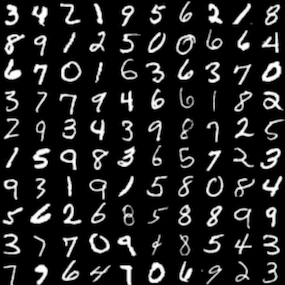
\includegraphics[width=\linewidth]{./Images/Chapter03/mnist_dataset.png}
  \endminipage\hfill
  \minipage{0.45\textwidth}%
    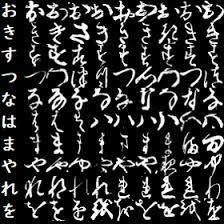
\includegraphics[width=\linewidth]{./Images/Chapter03/kuzushiji_mnist.jpg}
  \endminipage\hfill
  \caption{A visualization of two datasets that can be used for performing inductive transfer learning. On the left we represent instances of the popular MNIST dataset \cite{lecun1994mnist}, while on the right instances of the Kuzushiji-MNIST dataset \cite{clanuwat2018deep}. We see that both datasets share the same input space ($\mathcal{X}_S = \mathcal{X}_T$, black and white images), but are associated to different tasks ($\mathcal{T}_S \neq \mathcal{T}_T$, classification of digits vs classification of Japanese letters) and marginal distributions ($P_S(X)\neq P_T(X)$).}
  \label{fig:inductive_tl}
\end{figure*}


\paragraph{\textbf{\uppercase{T}ransductive \uppercase{T}ransfer \uppercase{L}earning}}
Also known as Domain Adaptation \cite{arnold2007comparative}, this type of TL is characterized by the fact that the source and target tasks are the same $\mathcal{T}_S = \mathcal{T}_T$, but their respective domains are different $\mathcal{D}_S \neq \mathcal{D}_T$. It is also possible that the feature spaces between domains are the same but, if that is the case, then the marginal probability distributions are different $P_S(X)\neq P_T(X)$. In its original formulation, \citet{arnold2007comparative} assumed that all unlabeled data in the target domain is available at training time. However, we hereafter report the definition of \citet{pan2009survey} who instead relax this condition and require only a subset of unlabeled target data to be seen at training time.
\begin{definition}
	Given a source domain $\mathcal{D}_S$ and a source task $\mathcal{T}_S$, and a target domain $\mathcal{D}_T$, and a target task $\mathcal{T}_T$, transductive transfer learning aims to help to improve the target predictive function $f_T(\cdot)$ in $\mathcal{D}_T$ by using the knowledge in $\mathcal{D}_S$ and $\mathcal{T}_S$, where $\mathcal{D}_S \neq \mathcal{D}_T$ and $\mathcal{T}_S = \mathcal{T}_T$. 
\end{definition}
As an example of transductive transfer learning let us assume that we would like to train a model to classify which type of clothing is depicted in an image. This time, differently from the inductive transfer learning case, the images in our target domain $\mathcal{D}_T$ are not black and white anymore, but rather colored images; therefore, defined over the RGB domain (see the right image of Fig. \ref{fig:transductive_tl}). We now assume that we have access to a pre-trained model which has already been trained to classify the same type of clothes, with the main difference being that the images constituting the source domain $\mathcal{D}_S$ were black and white images (see the left image of Fig. \ref{fig:transductive_tl}). If we now train this pre-trained model on our colored dataset, we see that our setting fits the transductive transfer learning scenario: our considered domains are different ($\mathcal{D}_S \neq \mathcal{D}_T$, black and white vs. colored images), but their respective tasks are the same  ($\mathcal{T}_S = \mathcal{T}_T$), since a model is always trained to classify types of clothing.

\begin{figure*}
 \minipage{0.45\textwidth}
    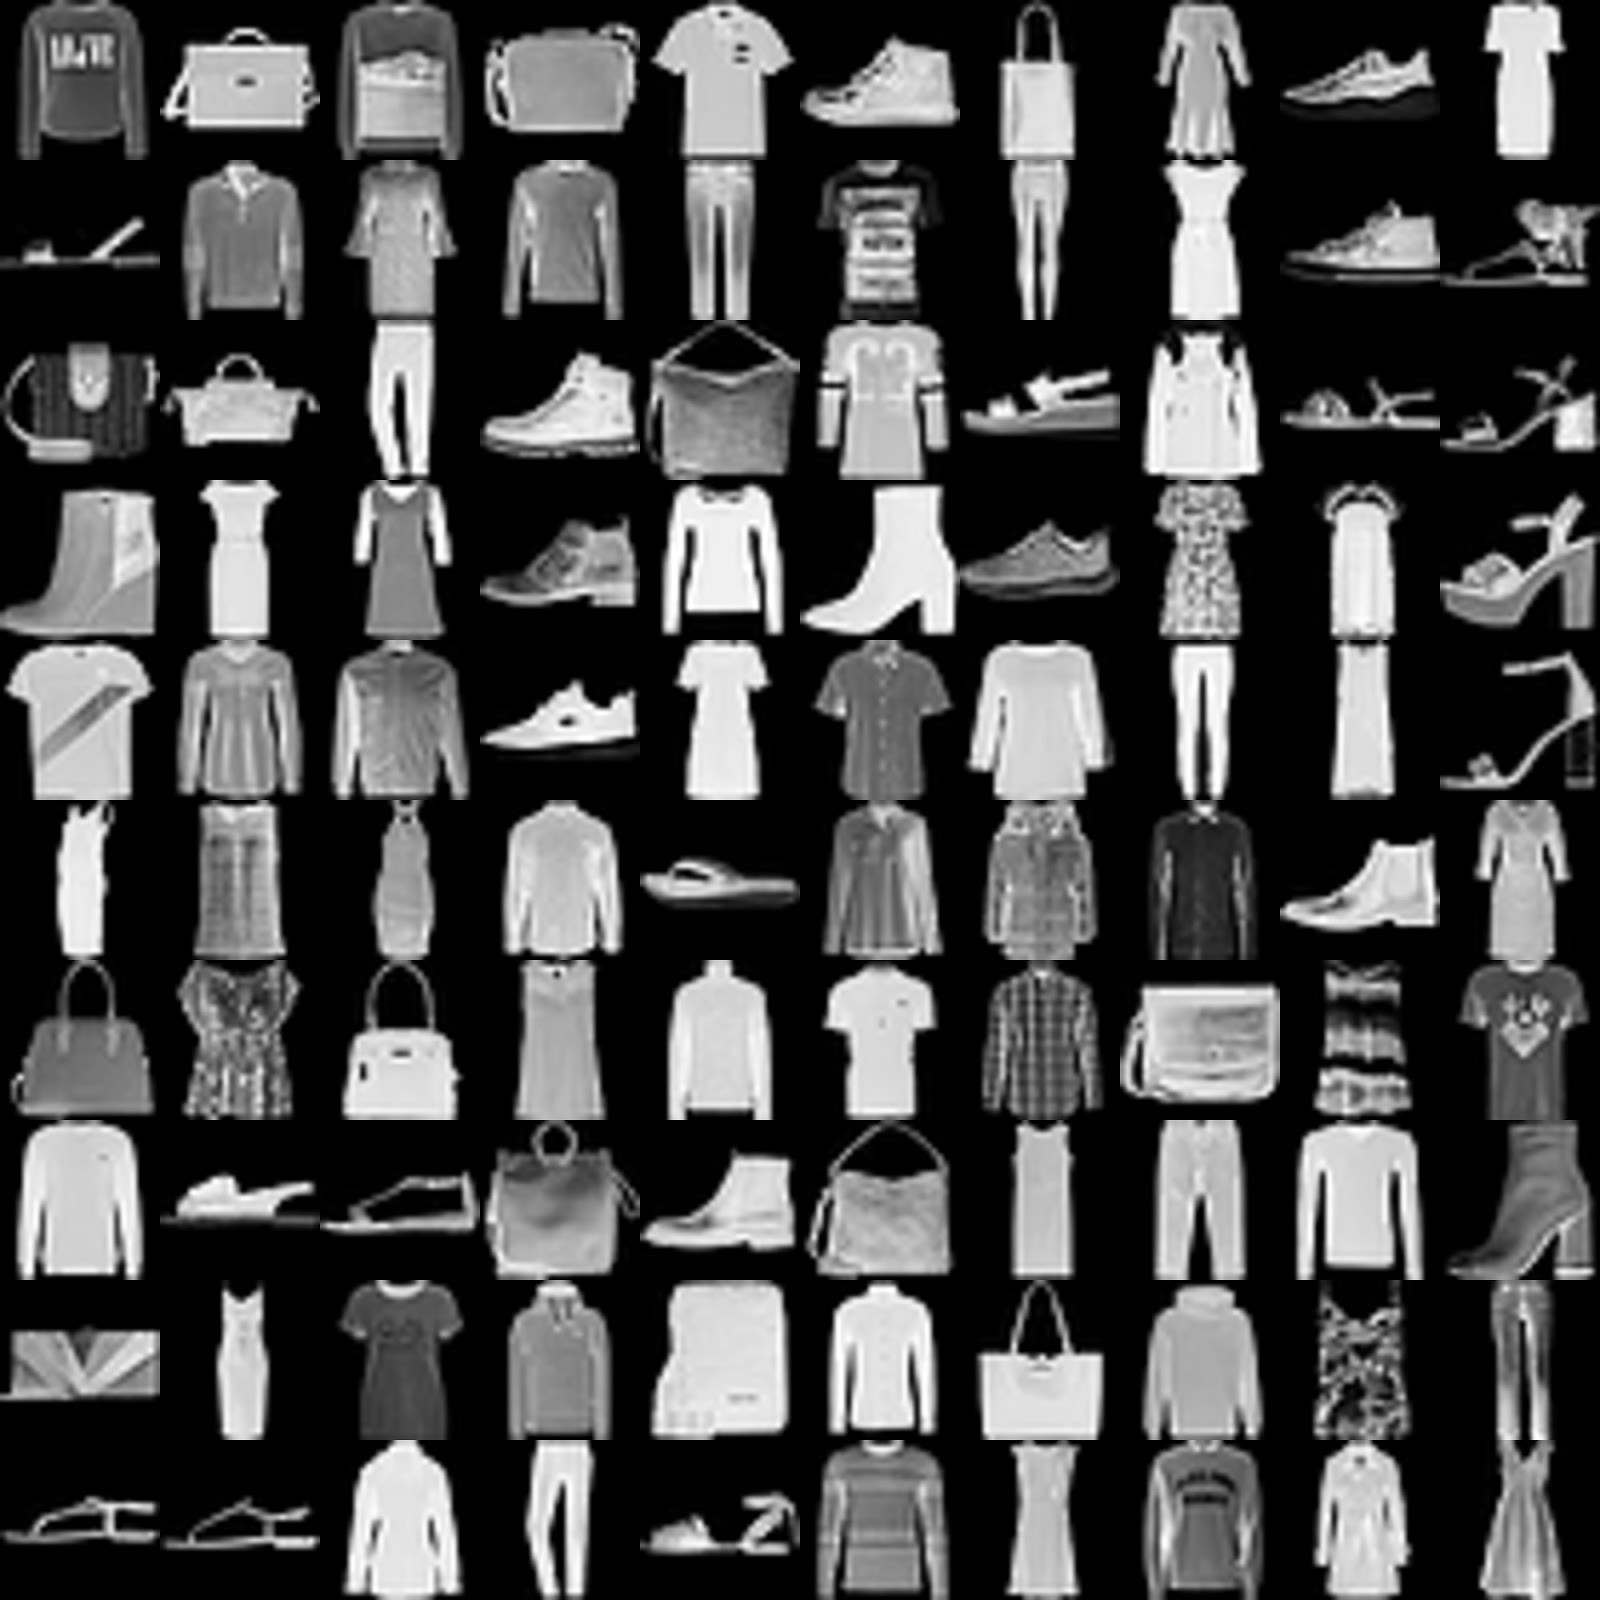
\includegraphics[width=\linewidth]{./Images/Chapter03/fashion_mnist}
  \endminipage\hfill
  \minipage{0.45\textwidth}%
    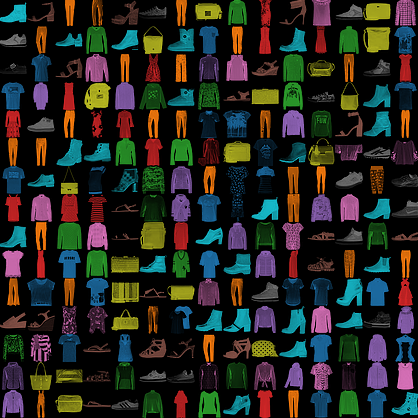
\includegraphics[width=\linewidth]{./Images/Chapter03/colorful_fashion_mnist}
  \endminipage\hfill
  \caption{Two datasets that are representative of transductive transfer learning. On the left we show images coming from the Fashion-MNIST dataset \cite{xiao2017fashion}, while on the right we report instances of the same dataset that are colored. In this case tasks among datasets are shared $\mathcal{T}_S = \mathcal{T}_T$ (classification of clothes), but the respective images come from different domains $\mathcal{D}_S \neq \mathcal{D}_T$ (black and white vs RGB images).}
  \label{fig:transductive_tl}
\end{figure*}

Although this section, as well as the second part of this dissertation, primarily focuses on supervised learning, we hereafter still report for the sake of completeness a definition of unsupervised transfer learning, and see how this kind of TL connects to the types of TL that we have analyzed so far.

\paragraph{\textbf{\uppercase{U}nsupervised \uppercase{T}ransfer \uppercase{L}earning}}
Arguably considered to be the most challenging and the least explored type of TL, unsupervised transfer learning is characterized by the total absence at training time of labeled data in both the source domain and the target domain. As mentioned by \citet{pan2009survey}, very little research work has so far explored this TL paradigm, with the only existing works exploring typical unsupervised learning topics such as clustering \cite{dai2008self, jin2011transferring, qian2015cluster} and dimensionality reduction \cite{wang2008transferred, zhu2013self, zhu2016robust}. Unsupervised transfer learning is defined as follows:
\begin{definition}
	Given a source domain $\mathcal{D}_S$ and a source task $\mathcal{T}_S$, and a target domain $\mathcal{D}_T$, and a target task $\mathcal{T}_T$, unsupervised transfer learning aims to help to improve the target predictive function $f_T(\cdot)$ in $\mathcal{D}_T$ by using the knowledge in $\mathcal{D}_S$ and $\mathcal{T}_S$, where $\mathcal{T}_S \neq \mathcal{T}_T$ and $\mathcal{Y}_S$ and $\mathcal{Y}_T$ are not observable. 
\end{definition}
Based on this definition, we can note that unsupervised transfer learning is more similar to inductive transfer learning than to transductive transfer learning as we again assume that the source and the target tasks are different $\mathcal{T}_S \neq \mathcal{T}_T$.


\subsection{Reinforcement Learning}
\label{sec:reinforcement_learning_tl}
When it comes to the Reinforcement Learning (RL) setup, the TL definition mentioned above slightly changes and becomes arguably less general. Recall from Chapter \ref{ch:reinforcement_learning} that in RL, the main goal is that of training an agent such that it becomes able to interact with its environment, a problem that is modeled with Markov Decision Processes (MDP). It follows that in the RL context, the previously introduced concept of domain $\mathcal{D}$ (which could come in numerous flavors) now comes in the arguably more strict form of an MDP $\mathcal{M}$. Just like domains, MDPs can either be representative of a source task, $\mathcal{M_S}$, or of a target task $\mathcal{M}_T$, with the latter case corresponding to the main RL problem we are interested in solving. The previously introduced predictive function $f(\cdot)$ now corresponds to the task of learning an optimal policy $\pi^*$ for $\mathcal{M}_T$. Based on these concepts, we give the following definition of TL for reinforcement learning that is adapted from the one proposed by \citet{zhu2020transfer}.

\begin{definition}
	Given a source MDP $\mathcal{M}_S$ and a target MDP $\mathcal{M}_T$, transfer learning in reinforcement learning aims to learn an optimal policy $\pi^{*}$ for $\mathcal{M}_T$ by exploiting some prior knowledge related to $\mathcal{M}_S$, denoted as $\mathcal{K}_S$, together with the knowledge that underlies $\mathcal{M}_T$, denoted as $\mathcal{K}_T$, such that:
	\begin{align}
		\pi^{*} = \argmax_{\pi} \mathds{E}_{s \sim\mu_{0}^{t},a\sim\pi}\bigl[Q^{\pi}_\mathcal{M}(s,a)\bigr],
	\end{align}
        %	where $\pi^* = \zeta(\mathcal{K}_S \sim \mathcal{M}_S, \mathcal{K}_T \sim \mathcal{M}_T): \mathcal{S}^t \rightarrow \mathcal{A}^t$ is a function mapping from the states to actions for $\mathcal{M}_T$ learned thanks to both $\mathcal{K}_S$ and $\mathcal{K}_T$.
	where $\pi^* = \zeta(\mathcal{K}_S, \mathcal{K}_T ): \mathcal{S}^t \rightarrow \mathcal{A}^t$ is a function mapping from the states to actions for $\mathcal{M}_T$ learned thanks to both $\mathcal{K}_S$ and $\mathcal{K}_T$.        
\end{definition}

Note that differently from the supervised learning case, we are now making explicit use of the concept of knowledge $\mathcal{K}$, which is what we would like to retain when moving from a source MDP $\mathcal{M}_S$ to a target MDP $\mathcal{M}_T$. We do this because RL is a machine learning paradigm that is arguably, more complex than supervised learning. A complexity that stems from the fact that in RL there are concepts such as e.g., rewards and policies, which are, by definition, not present in the supervised learning setup. As a result, $\mathcal{K}$ can come in forms that it cannot take in SL, and correctly identifying which kind of knowledge to transfer between $\mathcal{M}_S$ and $\mathcal{M}_T$ is just as important as developing a method that successfully transfers this knowledge in the first place. As mentioned by \citet{lazaric2012transfer} $\mathcal{K}$ can come in the following forms.

\paragraph{\textbf{\uppercase{T}ransfer of \uppercase{I}nstances}} In this scenario, $\mathcal{K}$ corresponds to RL trajectories coming in the form $\langle s_t, a_t, r_t, s_{t+1}\rangle$ and that have been collected on one, or possibly multiple, source MDPs $\mathcal{M}_S$. Such trajectories can then be used both in a model-based RL setting, as done by \citet{taylor2008transferring}, or for speeding up the process of learning a value function as described in \cite{lazaric2008transfer} and \cite{laroche2017transfer}. Ideally, transferring RL trajectories should result in highly sample efficient algorithms, although it is worth noting that this property, albeit desirable, can constrain the source task $\mathcal{M}_S$ and the target task $\mathcal{M}_T$ to have similar transition models and reward functions. This instance of TL is usually used within the batch RL setup, where gathering experience samples for $\mathcal{M}_T$ can be particularly expensive or time-consuming, which is a constraint that usually does not hold for $\mathcal{M}_S$. The typical challenge then consists of correctly identifying which of the samples coming from $\mathcal{M}_S$ are the most informative ones for solving $\mathcal{M}_T$, as for example, studied by \citet{tirinzoni2018importance}.

\paragraph{\textbf{\uppercase{T}ransfer of \uppercase{P}arameters}} As we have seen in Chapter \ref{ch:reinforcement_learning}, it is often desirable to integrate RL algorithms with parametric function approximators. The main goal is to then train these parametric functions to learn an approximation of an optimal value function or policy. When parameter transfer is performed, the main idea is to start solving the problem modeled by the target task $\mathcal{M}_T$ with a function that, instead of being initialized with random parameters, is initialized with parameters that have been learned on a certain source task $\mathcal{M}_S$. Examples of knowledge $\mathcal{K}$ that fit this description are the parameters $\theta$ of a pre-trained Deep Q-Network, or the parameters that model an Actor-Critic agent.  
\bigbreak
While both representations are arguably the most popular ones, it is important to mention that as described by \citet{tirinzoni2018transfer} there are alternative ways of representing $\mathcal{K}$. Among such ways, $\mathcal{K}$ can come in the form of e.g., features \cite{mehta2008transfer,barreto2017successor}, rewards \cite{konidaris2006autonomous,schaal2004estimating} and options \cite{singh2005intrinsically}.

\section{Deep Transfer Learning}
\label{sec:literature_review}

We now present the field of ``Deep Transfer Learning'' (DTL), a machine learning paradigm that aims at performing TL when a source model comes in the form of a pre-trained convolutional neural network. We start by describing how one can exploit the availability of a pre-trained network when training a model on the desired target task and then present a thorough literature review that describes the most successful applications that the DTL community has so far achieved.

\subsection{General Framework}
\label{sec:tl_general_framework}

Let us assume we would like to train a neural network on a regression task. Instead of initializing its weights randomly, we initialize it with weights that have already been optimized on a certain source task. We refer to the parameters of this pre-trained model as $\theta_S$, where $S$ stands again for ``source''. When training the network on the target task, the main challenge revolves around deciding up to what extent the parameters $\theta_S$ should be modified through stochastic gradient descent. In practice, this corresponds to deciding how much of the knowledge contained in $\theta_S$ should be retained when training the pre-trained network on $\mathcal{T}_T$. Typically, one can choose between three different approaches:

\begin{itemize}
	\item \textcolor{RoyalBlue}{Off-the-Shelf Extraction:} in this setting, the parameters $\theta_S$ of the pre-trained model are not changed when the network gets trained on the target task. Instead, the only weights that get optimized are the ones that are responsible for the final predictions of the model. In the regression example mentioned above, these weights would correspond to the ones parametrizing the network's final output neuron. Similarly, if we would be dealing with a classification problem, we would only train the weights that constitute the final softmax layer of the model, as this is the part of the network that, as described in Chapter \ref{ch:supervised_learning}, is responsible for outputting the predicted output classes. Since this approach does not involve any backpropagation operations, it is particularly desirable when computational resources are limited. In fact, one only needs to compute the forward pass in order to get the features from the pre-trained model. However, this approach also comes with the major limitation of not allowing the network to adapt to the target task as it assumes that all the knowledge that is required for solving $\mathcal{T}_T$ is already contained within $\theta_S$. In the context of convolutional neural networks, this corresponds to a model that has already learned all the features that are necessary for solving $\mathcal{T}_T$ when getting trained on $\mathcal{T}_S$.   

	\item \textcolor{RoyalBlue}{Fine-Tuning:} when this approach is adopted all the parameters $\theta_S$ that have been learned on the source task get optimized when training the network on the target task. Evidently, this training strategy is computationally more expensive than the previous one, as it involves all the training steps that characterize neural networks discussed in Chapter \ref{ch:supervised_learning}. Despite being computationally more demanding, fine-tuning a network has the significant benefit of allowing a model to become target task-specific. In fact, whilst training, part of the knowledge contained within $\theta_S$ can be ``forgotten'', which will result in a new set of parameters, $\theta_T$, that can perform better on $\mathcal{T}_T$ than $\theta_S$. From a practical perspective, however, it is important to train the model in such a way that the knowledge contained within $\theta_S$ does not get ``forgotten'' too quickly, while at the same time ensuring that the network stays flexible enough for successfully learning the target task. One possible way of achieving this is by using small learning rate values for training.      

	\item \textcolor{RoyalBlue}{Intermediate Approaches:} the aforementioned approaches do either not modify the source weights $\theta_s$ parametrizing the convolutional layers at all, or instead allow the network to completely change them. However, some intermediate approaches are also possible. As convolutional networks typically come with a large number of layers, one possible way of exploiting the respective source weights $\theta_s$ could be done by fine-tuning only a specific sub-set of layers, while keeping the remaining ones frozen. As a result only one part of the model will involve the backpropagation algorithm, whereas the remaining parts will simply act as feature extractors. Furhtermore it is also worth noting that an off-the-shelf feature extraction approach can technically be performed after any convolutional layer. As features can be obtained after any convolutional layer, some intermediate approaches rely on extracting them without performing a forward pass throughout the entire network. While such approaches can certainly be valuable \cite{mormont2018comparison,sasso2021fractional}, they will not be considered throughout this thesis. 


\end{itemize}

While all approaches come with pros and cons, the second option is usually preferred if enough computational resources are available. In fact, as we will see in the coming section, the community seems to agree that it often results into better final performance. When DTL strategies are adopted, it is usually good practice to compare the performance of a pre-trained model with the performance that is obtained by a model that is initialized randomly, and that gets therefore trained from scratch. Throughout this thesis we will constantly characterize the benefits of adapting TL strategies from this perspective, therefore, to add even more clarity to the concepts presented in this section, we also visually represent them in Fig. \ref{fig:network_training_approaches}. 

\begin{figure*}[!htb]
\minipage{0.3\textwidth}
  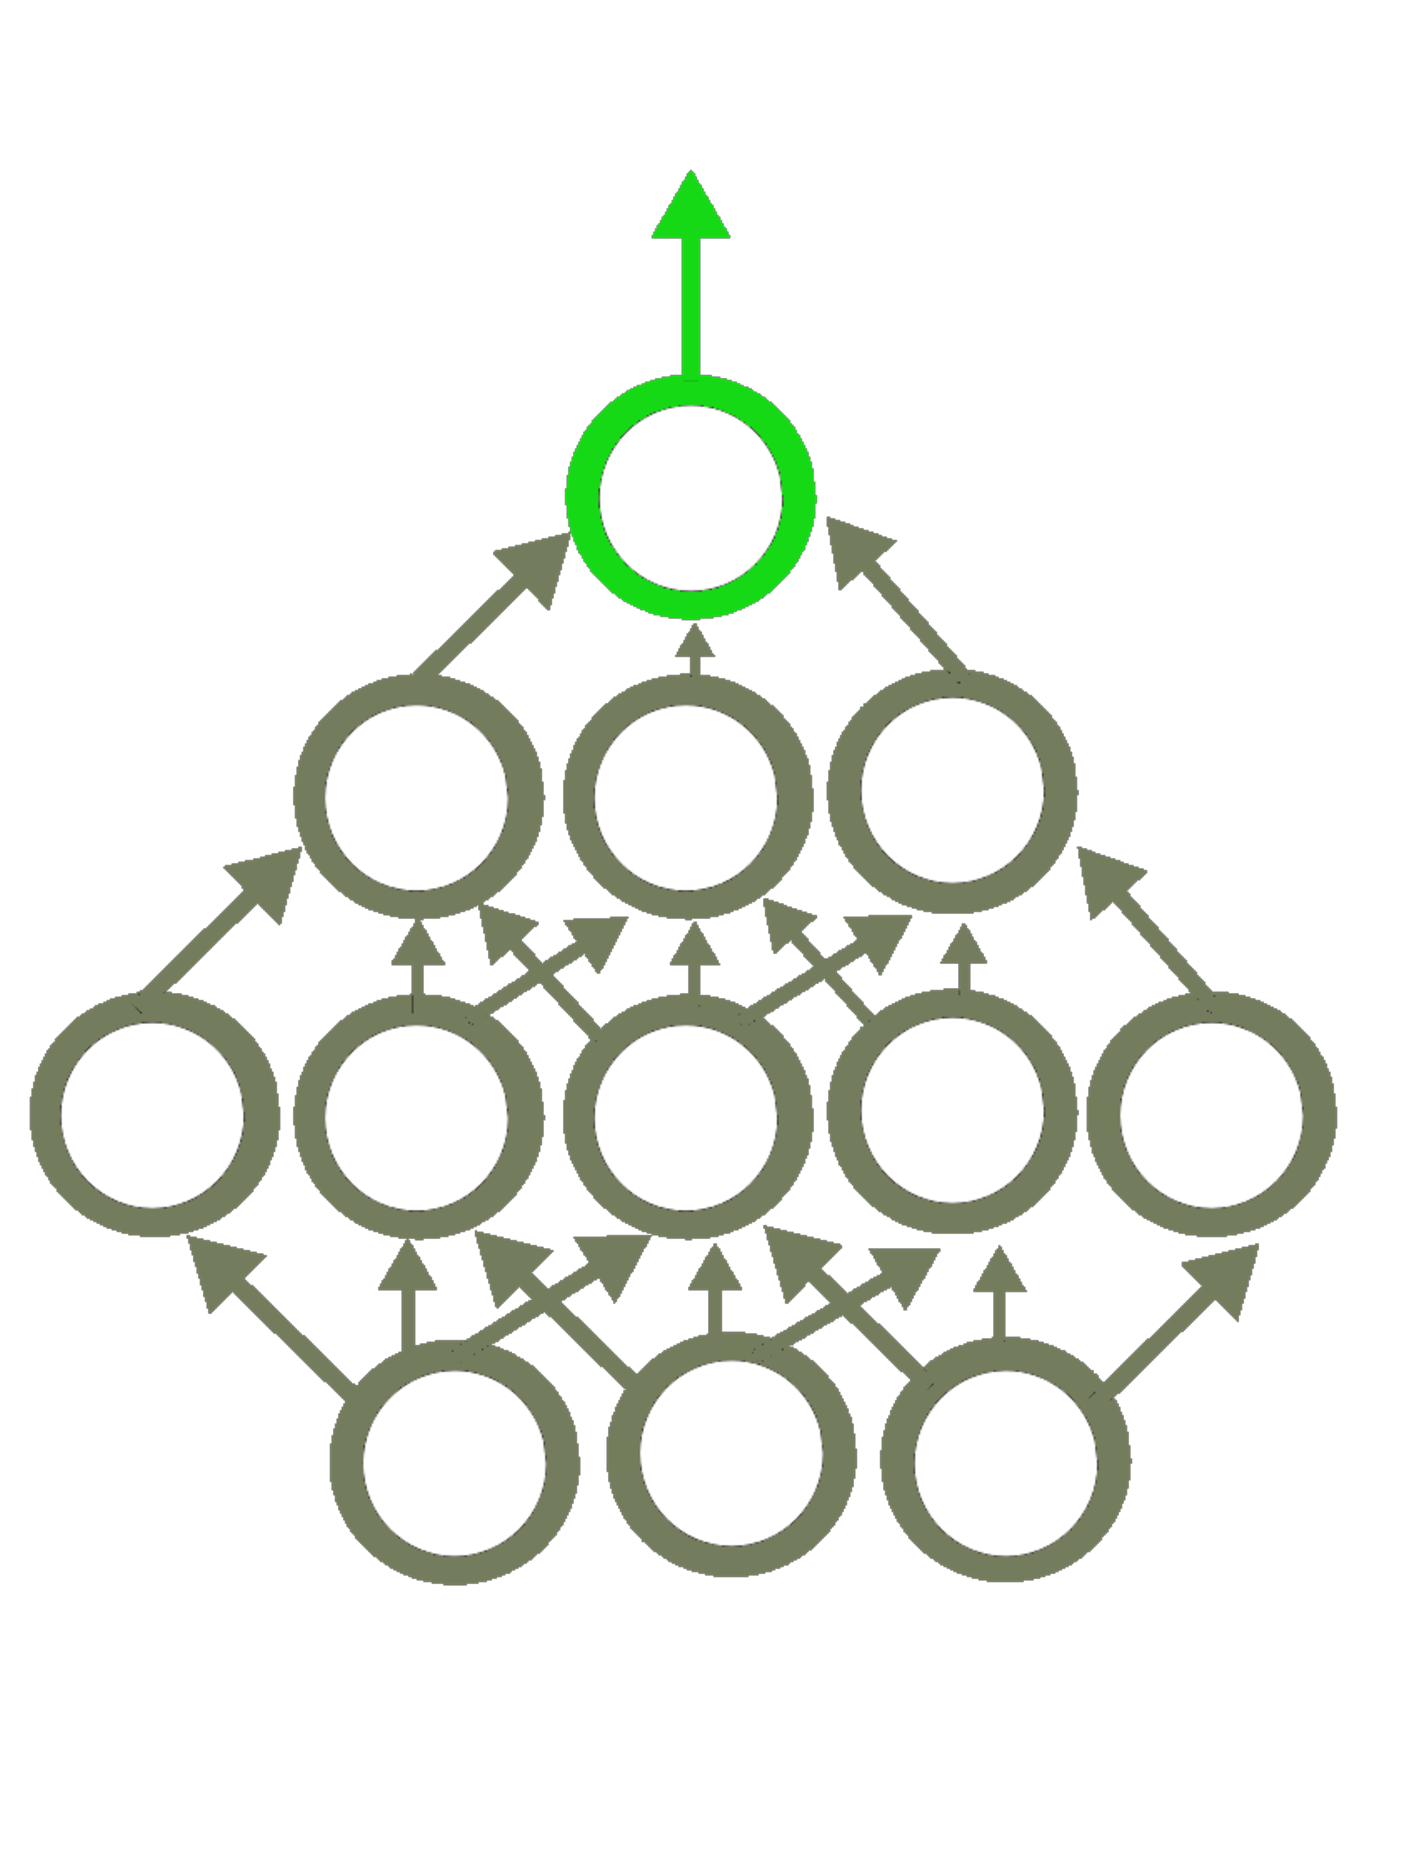
\includegraphics[width=\linewidth]{./Images/Chapter04/frozen_net.pdf}
\endminipage\hfill
\minipage{0.3\textwidth}
  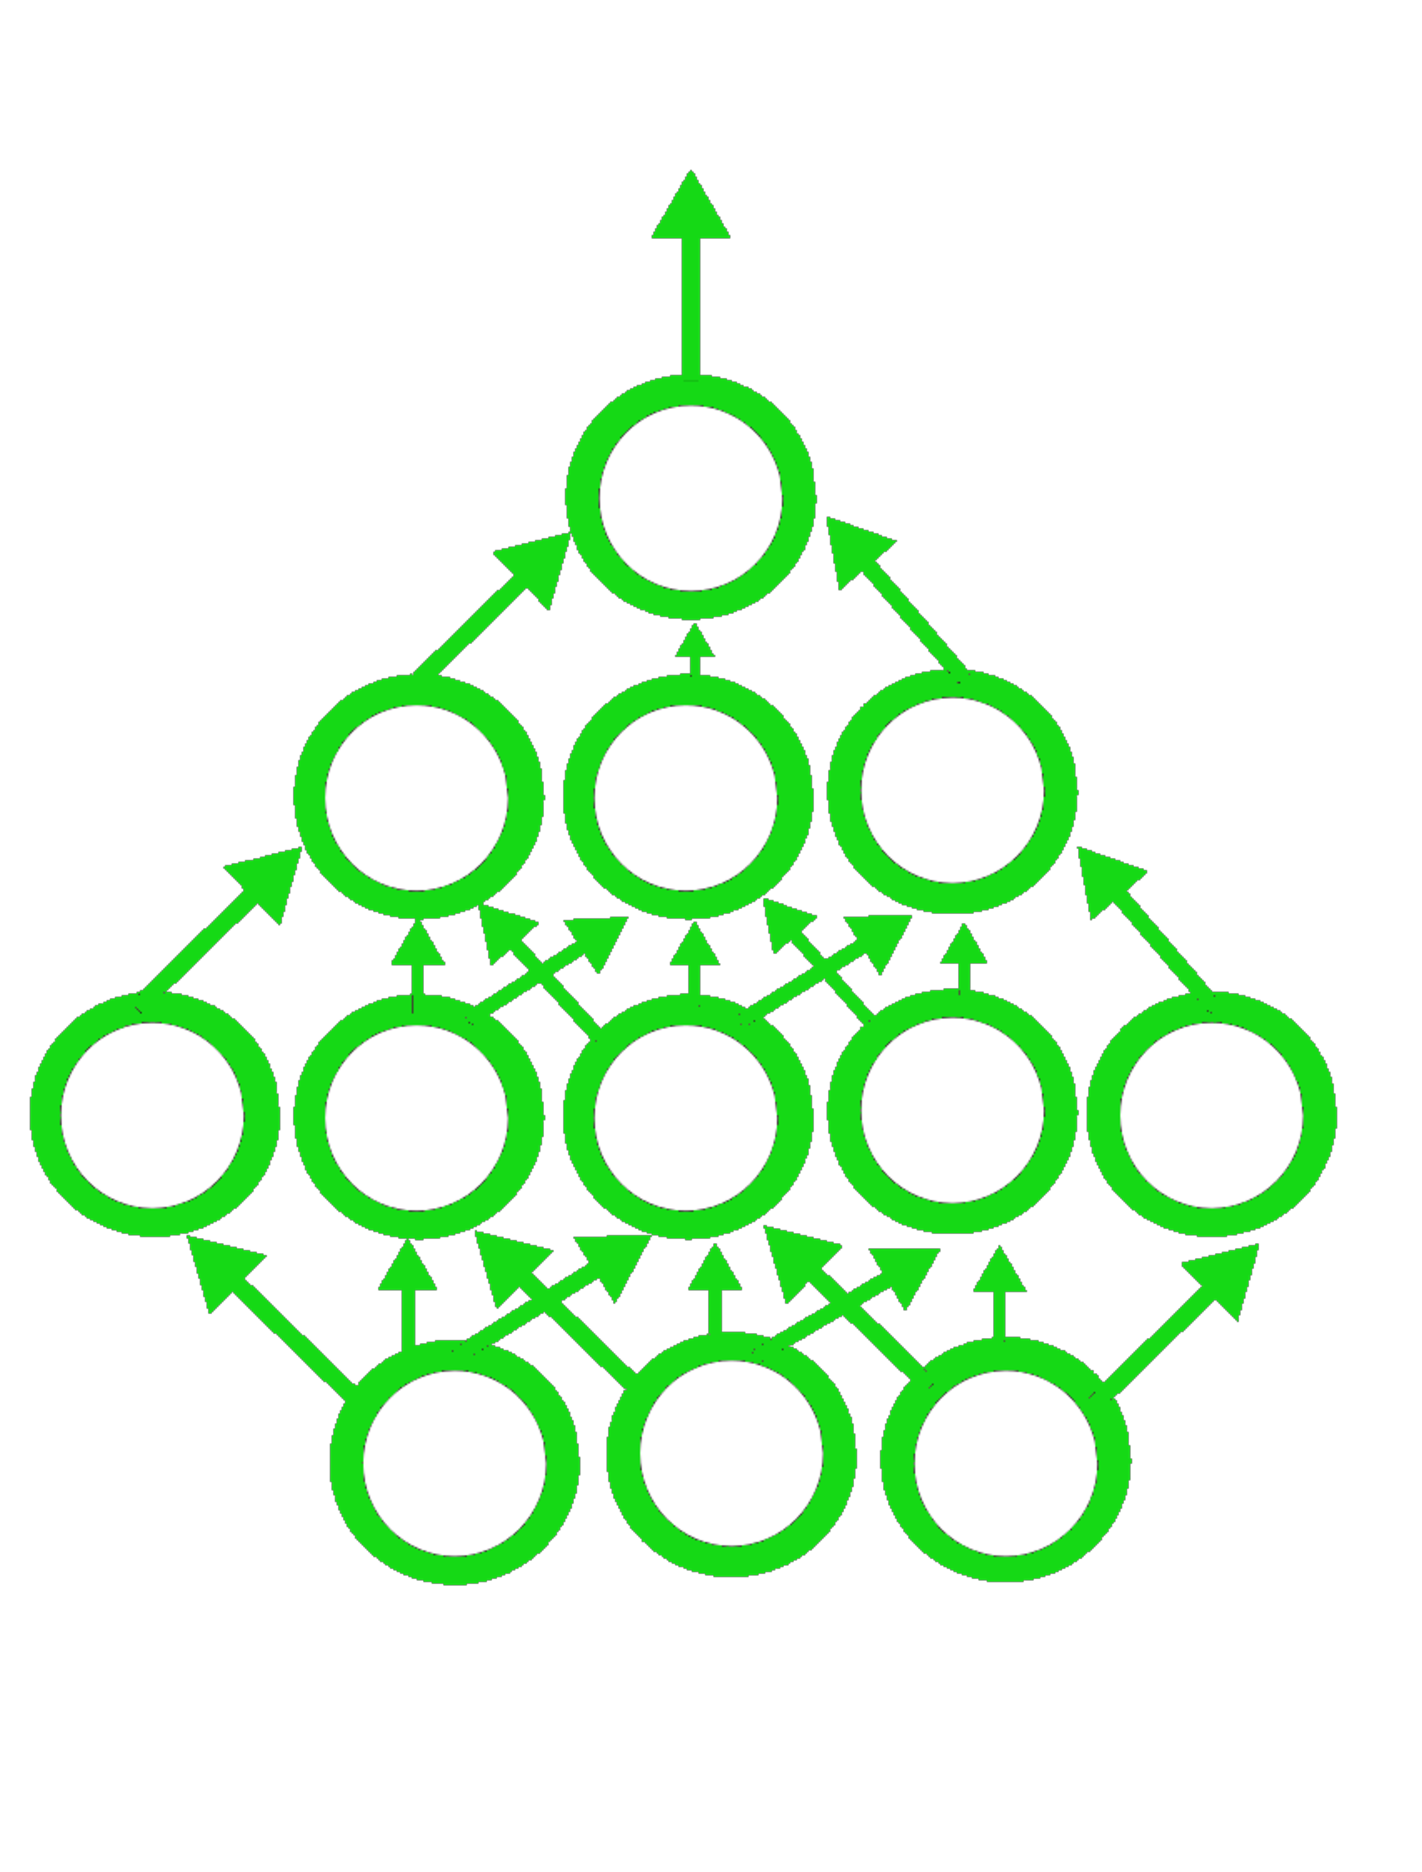
\includegraphics[width=\linewidth]{./Images/Chapter04/fine_tuning_net.pdf}
\endminipage\hfill
\minipage{0.3\textwidth}%
  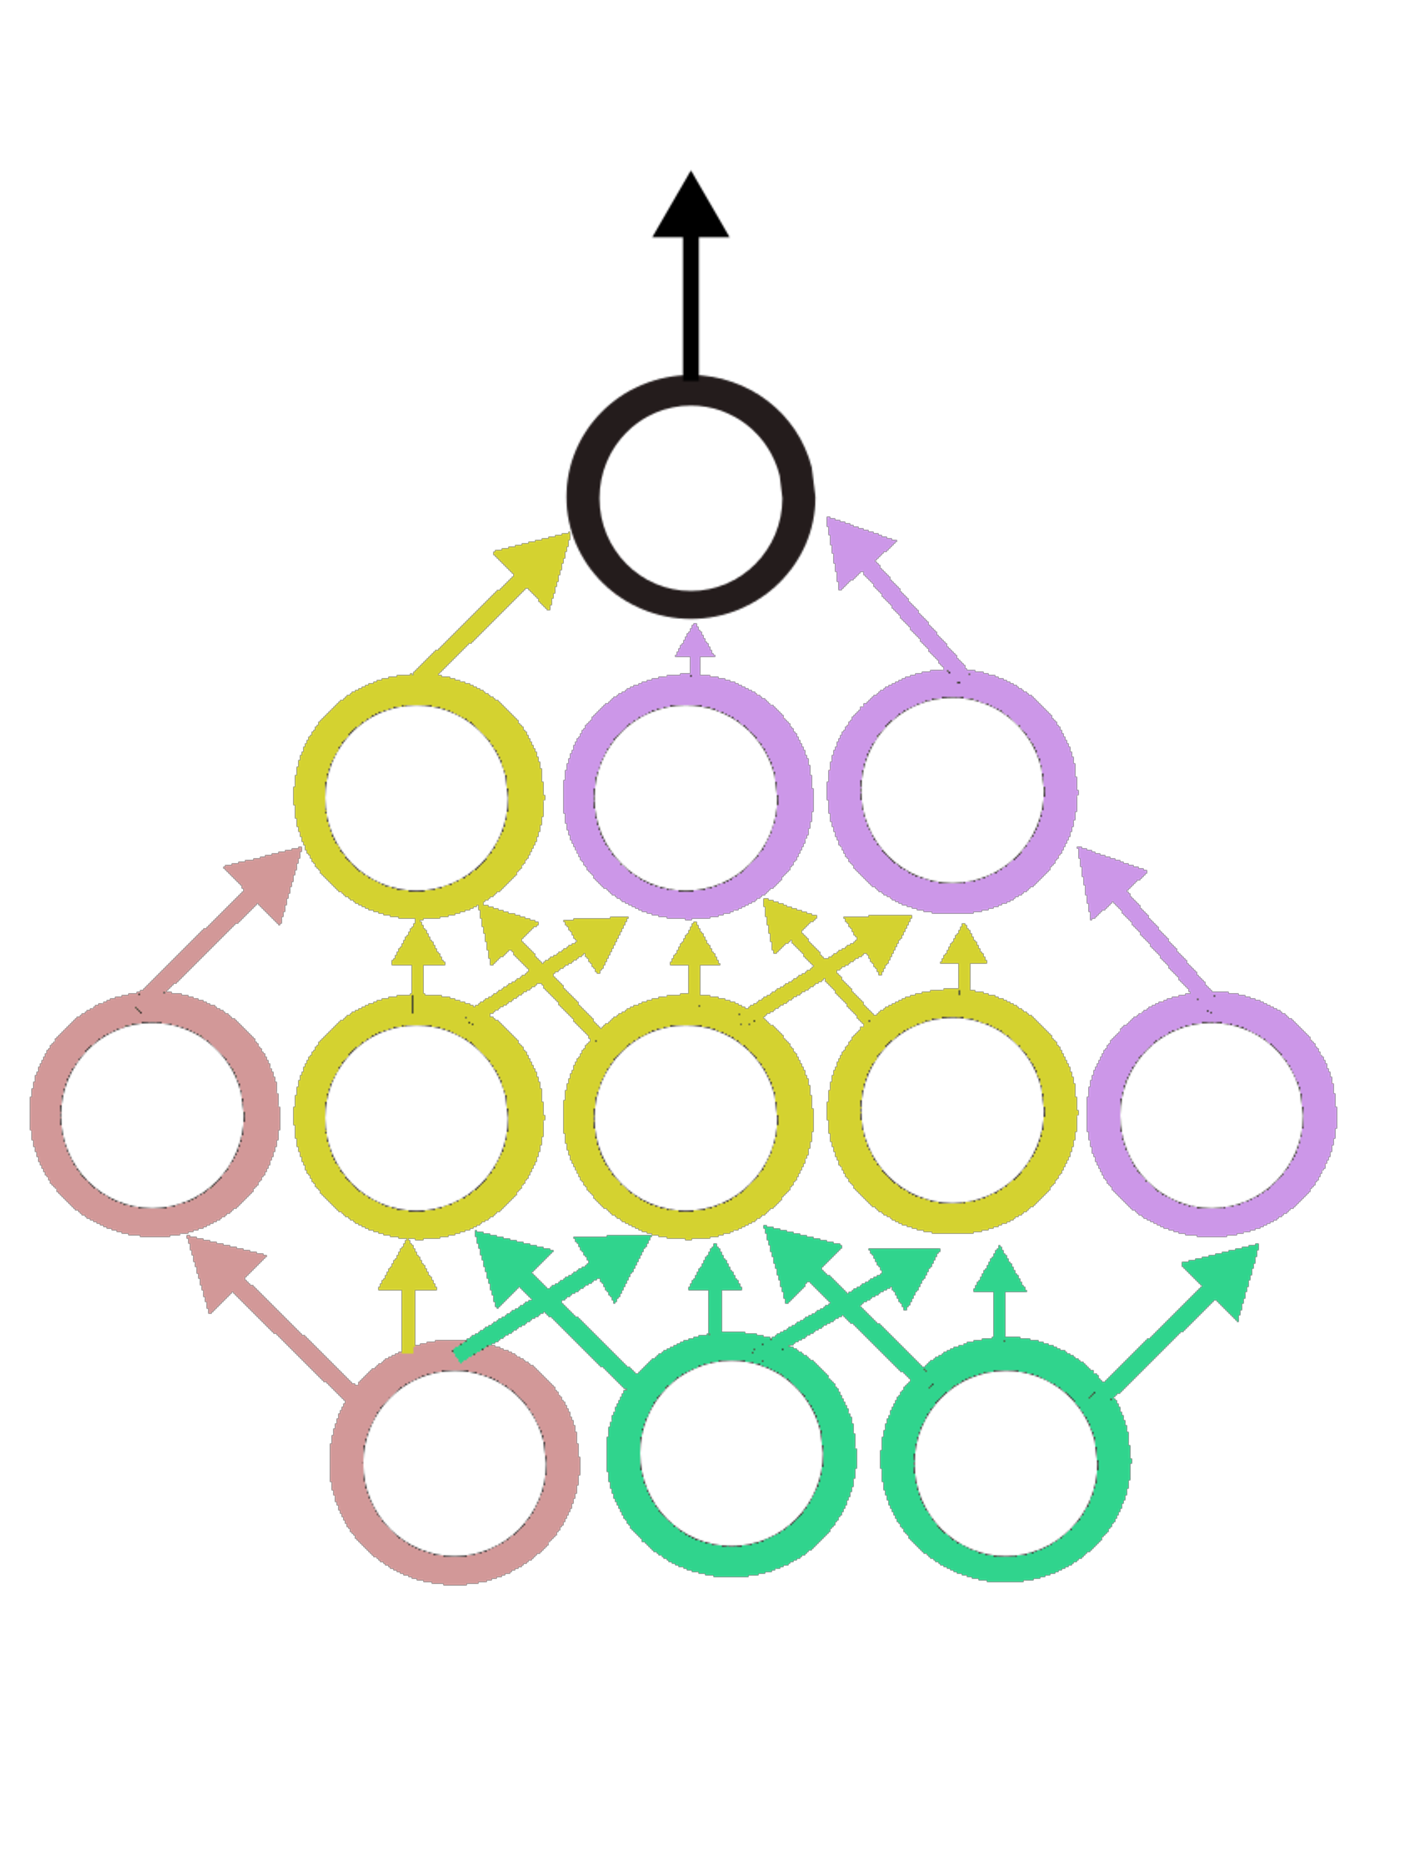
\includegraphics[width=\linewidth]{./Images/Chapter04/random_net.pdf}
\endminipage
\caption{A simplified visual representation of the different deep transfer learning training paradigms that are considered throughout this thesis. The first plot represents a model that comes as pre-trained on a source task but which will not update most of its weights during the training stage (represented in gray): the only trainable parameters of this network are the ones that parametrize the final layer of the model and that are represented in green. In the second plot we visually represent a model that is parametrized with weights that have been learned on a certain source task, and that get ``unfrozen'' when the network gets trained on the target task, therefore defining the model as fully trainable. Lastly we visualize a model that does not come as pre-trained on any source task, and that is therefore initialized with random weights instead (represented by the various colours). As already mentioned throughout this chapter, the main goal of TL is to obtain a model that if trained with the first two approaches results into a final performance that is better than the one that would be obtained by the last type of model.}
\label{fig:network_training_approaches}
\end{figure*}


\subsection{Literature Review}
\label{sec:literature_review_ch03}

We now review how the deep transfer learning community has over the years studied the transfer learning properties of convolutional neural networks. Specifically, we focus on four different perspectives.

\paragraph{\textbf{\uppercase{C}onvolutional \uppercase{N}eural \uppercase{N}etworks as \uppercase{F}eature \uppercase{E}xtractors}}
As soon as convolutional neural networks started to perform well on popular Computer Vision (CV) benchmarks, research investigating whether these networks could be transferred and reused for novel tasks started to bloom. The first work exploring this direction was that of \citet{yosinski2014transferable}, who observed that the early layers of deep neural networks trained on natural images, learn features which are general and, therefore, independent from the CV task used for training. Such generalization property can hence be exploited by initializing a convolutional neural network with transferred features instead of randomly, which is a strategy that results in models less prone to overfitting. 

Alongside \citet{yosinski2014transferable}, \citet{donahue2014decaf} investigated whether features extracted from a convolutional neural network trained for image classification could also be used for tackling CV tasks such as scene recognition and domain adaptation. \citet{donahue2014decaf} showed that this was indeed the case and publicly released the pre-trained model under the name of \texttt{DeCAF} intending to stimulate the CV community to investigate further the extent to which the features learned by this network were transferable to novel tasks. Almost concurrently, similar conclusions about the transferability of pre-trained convolutional networks were drawn by \citet{oquab2014learning}, who showed the benefits of using a pre-trained convolutional model as feature extractor when dealing with object and action localization problems, and by \citet{zeiler2014visualizing} who first showed that on many problems it was more beneficial to simply train the final classification layer of a pre-trained network, than to train a randomly initialized model from scratch. While definitely promising, all these works restricted their experimental analysis to a relatively small set of CV problems, and it was only with the seminal work of \citet{sharif2014cnn} that the deep learning community realized how powerful pre-trained networks could be. \citet{sharif2014cnn} used the off the shelf (OTS) features of the pre-trained \texttt{OverFeat} network \cite{sermanet2013overfeat} for tackling numerous challenging CV problems and consistently reported a final performance that was superior to the one of the state of the art algorithms of the time. Next to providing a wealth of empirical evidence supporting the use of off-the-shelf features, their work also established the first training protocol for combining high dimensional OTS features with linear classifiers, such as SVMs, and dimensionality reduction techniques such as principal component analysis. 

It did not take long before the scientific community started to investigate whether off-the-shelf features could also be used for problems outside the typical CV benchmarks, and therefore fully realized the potential of this TL approach. Among the very first practical applications, we mention the work of \citet{van2015off} who used the previously mentioned \texttt{DeCAF} model for (successfully) tackling the challenging medical task of pulmonary nodule detection. Along the same line of research, equally good results were obtained within the medical domain by \citet{hernandez2018periocular} who tackled the problem of periocular recognition, and by \citet{nguyen2017iris} who considered the similar task of iris recognition.

Further successful applications of OTS classification, which go beyond the medical domain, are the ones reported by \citet{sharma2015adapting}, who considered the handwriting recognition task of word spotting, and the one of \citet{van2015deep}, who studied the task of gender classification. While all these researches solely relied on an OTS feature extraction approach when addressing a CV problem, it is also worth noting that OTS features can be used in combination with more traditional CV feature engineering techniques such as SIFT \cite{lowe2004distinctive} and HOG \cite{dalal2005histograms}. This research direction has been successfully explored by, e.g., \citet{wang2014action} who examined the task of human action understanding, and by \citet{zhong2016face} who addressed the problem of face localization.


\paragraph{\textbf{\uppercase{O}n the \uppercase{B}enefits of \uppercase{F}ine-\uppercase{T}uning}}
Modern deep learning frameworks such as \texttt{TensorFlow} \cite{abadi2016tensorflow} and \texttt{PyTorch} \cite{paszke2017automatic}, provide high level and easy to use APIs that make it possible to create and train deep learning models even without a necessarily strong machine learning background. Among the main reasons that have made deep learning so accessible there is the fact that the aforementioned deep learning libraries provide easy access to models that have already been trained on a large variety of CV tasks \cite{russakovsky2015imagenet, lin2014microsoft, everingham2010pascal}. As a result, using pre-trained neural networks has become increasingly easy, which is among the reasons that allowed the deep learning community to explore whether fine-tuning pre-trained models could result in better performance than simply using them as OTS feature extractors. It is easy to see how this research question is of high practical interest and why it has therefore been heavily explored by practitioners working at the intersection of machine learning and fields such as medicine \cite{tajbakhsh2016convolutional,ho2021evaluation}. Among the first works exploring whether it is beneficial to fine-tune pre-trained models instead of using them as simple feature extractors, there is the one of \citet{tajbakhsh2016convolutional}. The authors consistently show that fine-tuning a pre-trained network outperforms the OTS feature extraction approach when it comes to four distinct medical imaging tasks and that, similarly to what was predicted by \citet{zeiler2014visualizing}, pre-trained networks outperform models that are trained from scratch. A similar conclusion has also been reached by \citet{mormont2018comparison}, who analyzed the same research question under the lens of image classification problems coming from the digital pathology field. They also show that fine-tuning yields better performance than OTS feature extraction, but they do not answer whether this TL strategy works better than training a network from scratch. The question of whether to fine-tune or not to fine-tune a neural network has also been explored outside of the CV domain. Among the different works, we mention the one of \citet{peters2019tune}, who address this question from a Natural Language Processing (NLP) perspective. In line with what has been observed by the CV community, they also highlight the significant benefits that can come from fine-tuning popular NLP models such as ELMo \cite{peters2018deep} and BERT \cite{devlin2018bert} as long as the source task is carefully chosen. By now, studies investigating the benefits coming from fine-tuning pre-trained models are countless and range over a large variety of domains that do not necessarily strictly involve CV problems \cite{ackermann2018using,dominguez2019transfer,george2017deep,boulanger2013audio,deng2013new,kong2020panns,zarrella2016mitre,howard2018universal,houlsby2019parameter}.


\paragraph{\textbf{\uppercase{O}n the \uppercase{R}ole of \uppercase{I}mageNet as \uppercase{S}ource \uppercase{T}ask}} Throughout this chapter, we have constantly referred to the concept of source domain $\mathcal{D}_S$ and source task $\mathcal{T}_S$, two key elements without which the entire field of TL would not even exist. Albeit in the previous paragraphs we have mentioned the task of image classification as source task $\mathcal{T}_S$ that can be used for pre-training convolutional networks, we have not explicitly described what this task consists of in practice. When adopting TL strategies for CV problems, the most common and, by far successful, approach is that of relying on models that have been trained for the ImageNet Large Scale Visual Recognition Challenge (ILSVRC) \cite{russakovsky2015imagenet}. The ILSRVC dataset, more commonly referred to as the ImageNet dataset, is a collection of over one million natural images that are categorized among one thousand different classes. Until 2017 it was primarily considered to be the most complex and challenging problem of all CV and is among the main reasons which have encouraged the deep learning community to develop most of the neural architectures that we described in Chapter \ref{ch:supervised_learning}. Due to the large number of samples constituting the dataset and the complexity of the tackled task, networks trained for the ILSVRC challenge are regularly used as pre-trained networks even when the target task $\mathcal{T}_T$ does not involve the classification of natural images. Intuitively, the reasons behind this choice are very straightforward: on the one hand, it is safe to assume that some of the features that are learned by a network that receives as input more than one million images will, at least in part, correspond to the features that the same network would have to learn when getting trained from scratch on the desired target task.

On the other hand, it is also unlikely that the target task $\mathcal{T}_T$ will be more complex than the source task $\mathcal{T}_S$ since it is not common to deal with classification problems that involve more than 1000 classes. In this sense, as pointed out by \citet{mensink2021factors}, it is reasonable to assume that if a network performs well on $\mathcal{T}_S$, it should also perform well on $\mathcal{T}_T$, as the latter task is essentially easier than the former. Despite these intuitive explanations, a large body of work has studied why it is beneficial to transfer ImageNet pre-trained models and the factors of influence of this dataset for TL. This question was first tackled by \citet{huh2016makes} who studied, among other questions, how many examples and classes of the ImageNet dataset should be used for successfully pre-training a model. Perhaps surprisingly, they found that already half of the ImageNet data yielded a well-performing pre-trained network and that among the different 1000 classes, it was already enough to pre-train a network on a subset of 127 of them. \citet{kornblith2019better} empirically studied the benefits of using ImageNet pre-trained models for 12 different classification problems and found that the better a model performs on ImageNet, the better it transfers to new unseen tasks. A similar study, which, however, yielded slightly different results, is the one of \citet{he2019rethinking} who showed that there might not be significant differences in terms of final performance between using an ImageNet pre-trained network and a randomly initialized one, but that the first ones consistently converge faster than the latter. Finally, the recent work of \citet{mensink2021factors} shows that ImageNet pre-trained models always outperform models that are trained from scratch, but that this dataset might not necessarily always be the best possible source task for pre-training. It is worth noting that all the examples mentioned earlier revolve around the field of supervised learning within CV, it naturally follows that different pre-training strategies, and therefore different source domains, need to be considered for other fields (see e.g. NLP.). Since discussing these techniques would go beyond the main scope of this dissertation, we do not present them here. However, we refer the reader to \cite{mikolov2013efficient,rosset2020knowledge,brown2020language,devlin2018bert} for a discussion of pre-training strategies outside the CV and supervised learning domain.

\paragraph{\textbf{\uppercase{T}he \uppercase{D}eep \uppercase{R}einforcement \uppercase{L}earning \uppercase{S}etting}}
While within the supervised learning setting, the body of work studying the transfer learning properties of neural networks is substantial, the same cannot be said when it comes to reinforcement learning. Although, as presented in Sec. \ref{sec:reinforcement_learning_tl} there exist many different approaches for performing TL in RL, the integration of such techniques with convolutional neural networks is much rarer. Perhaps the work that studies the TL properties of Deep Q-Networks in a flavor that is the closest to the TL approaches used in supervised learning presented in Fig. \ref{fig:network_training_approaches} is that of \citet{farebrother2018generalization}. The authors study whether convolutional neural networks that are trained with the DQN algorithm \cite{mnih2015human} are capable of learning features that are robust enough to allow the algorithm to generalize across different tasks. The results, obtained on four different Atari 2600 games do not provide a clear answer to this question: when Deep Q-Networks come as pre-trained on a particular game and simply get fine-tuned on a new different game, the authors do not observe any of the benefits that this TL approach typically yields in the supervised learning context. However, if networks get pre-trained in combination with typical supervised learning regularization techniques such as dropout \cite{srivastava2014dropout} and $l_2$ regularization, then the authors observe that fine-tuning these models results in a final performance that is better than the one of models trained from scratch. While indeed encouraging, these results were only obtained on a minimal set of RL environments, and it is unclear whether these conclusions would hold if a more extensive set of benchmarks, and algorithms, would be tested. A similar study, which arguably presents the same limitations, is the one performed by \citet{tyo2020transferable}. On the same line with \citet{farebrother2018generalization}, the authors study the effect of fine-tuning different pre-trained Rainbow agents \cite{hessel2018rainbow} that use different weight initialization strategies. Results reported on three different Atari games show that fine-tuning is beneficial only for one single game but do not explain the TL properties of pre-trained Deep Q-Networks any further. A more thorough and successful study is the one presented by \citet{parisotto2015actor}, where the authors also investigate the effect of fine-tuning pre-trained DRL agents and show that this TL strategy can result in significant benefits. Their study, however, presents some significant differences when compared to the previous works. First, the DRL algorithm under scrutiny is a policy gradient algorithm which, as discussed in Chapter \ref{ch:reinforcement_learning}, is part of a family of techniques that is significantly different from the family that DQN and Rainbow are part of. Second, their proposed Actor-Mimic algorithm does not come as pre-trained on a single Atari game anymore but is pre-trained in a multi-task learning setting instead. The algorithm, therefore, deals with different source-tasks $\mathcal{T}_S$ during the pre-training stage, which is a strategy that arguably can result in algorithms that are more robust and suitable for TL \cite{kirkpatrick2017overcoming}.  


\section{Relevance for this Dissertation}
\label{sec:relevance}

With all the concepts above and the ones presented in Chapters \ref{ch:supervised_learning} and \ref{ch:reinforcement_learning}, we are now ready to end this first part of this dissertation by describing how all the aforementioned content will play a role throughout the rest of this thesis. 


\begin{takeaway}{Takeaway of Part I}
First, we start by noting that all the quantitative results that will be presented from now on will be defined with respect to the three transfer learning benefits that we described in Sec. \ref{sec:rationale}. No matter which kind of task we will be training neural networks for, we will always seek to identify at least one of the three possible transfer learning benefits. The only chapter where we will not do this is Chapter \ref{ch:dqv_family_of_algorithms}, which instead, will serve for introducing some novel deep reinforcement learning algorithms that will be studied from a transfer learning perspective only in Chapter \ref{ch:dqn_transfer}.

When it comes to the research performed within the supervised learning setting (Chapters \ref{ch:tl_natural_to_non_natural}, \ref{ch:minerva} and \ref{ch:tl_lth}), it is important to note that we will only consider the inductive transfer learning scenario. More specifically, we will always study the extent to which neural networks pre-trained on natural images can generalize to non-natural datasets. The content of these datasets, and therefore the considered target tasks $\mathcal{T}_T$, will change from chapter to chapter, and so will the source task $\mathcal{T}_S$ that will be used for pre-training. For the research involving reinforcement learning, we will instead only consider the TL setting that studies the transferability of parameters (Chapter \ref{ch:dqn_transfer}) presented in Sec. \ref{sec:reinforcement_learning_tl}. As a result, no matter whether we will tackle supervised learning problems or reinforcement learning ones, the experimental protocol that we will adopt will always follow the TL training strategies that we have described in Sec. \ref{sec:tl_general_framework} and presented in Fig. \ref{fig:network_training_approaches}. As a result, the respective studies will all contribute to the development of the field that studies the transferability of neural networks that we have reviewed in Sec. \ref{sec:literature_review}.
\end{takeaway}

We will now present our research investigating the TL properties of convolutional neural networks trained for supervised learning problems.
